\documentclass[letter, 11pt]{article}
%% ================================
%% Packages =======================
\usepackage[utf8]{inputenc}      %%
\usepackage[T1]{fontenc}         %%
\usepackage{lmodern}             %%
\usepackage[spanish]{babel}      %%
\decimalpoint                    %%
\usepackage{fullpage}            %%
\usepackage{fancyhdr}            %%
\usepackage{graphicx}            %%
\usepackage{amsmath}             %%
\usepackage{color}               %%
\usepackage{mdframed}            %%
\usepackage[colorlinks]{hyperref}%%
%% ================================
%% ================================

%% ================================
%% Page size/borders config =======
\setlength{\oddsidemargin}{0in}  %%
\setlength{\evensidemargin}{0in} %%
\setlength{\marginparwidth}{0in} %%
\setlength{\marginparsep}{0in}   %%
\setlength{\voffset}{-0.5in}     %%
\setlength{\hoffset}{0in}        %%
\setlength{\topmargin}{0in}      %%
\setlength{\headheight}{54pt}    %%
\setlength{\headsep}{1em}        %%
\setlength{\textheight}{8.5in}   %%
\setlength{\footskip}{0.5in}     %%
%% ================================
%% ================================

%% =============================================================
%% Headers setup, environments, colors, etc.
%%
%% Header ------------------------------------------------------
\fancypagestyle{firstpage}
{
  \fancyhf{}
  \lhead{
\includegraphics[height=4.5em]{LogoDFI.jpg}}
  \rhead{FI3104-1 \semestre\\
         Métodos Numéricos para la Ciencia e Ingeniería\\
         Prof.: \profesor}
  \fancyfoot[C]{\thepage}
}

\pagestyle{plain}
\fancyhf{}
\fancyfoot[C]{\thepage}
%% -------------------------------------------------------------
%% Environments -------------------------------------------------
\newmdenv[
  linecolor=gray,
  fontcolor=gray,
  linewidth=0.2em,
  topline=false,
  bottomline=false,
  rightline=false,
  skipabove=\topsep
  skipbelow=\topsep,
]{ayuda}
%% -------------------------------------------------------------
%% Colors ------------------------------------------------------
\definecolor{gray}{rgb}{0.5, 0.5, 0.5}
%% -------------------------------------------------------------
%% Aliases ------------------------------------------------------
\newcommand{\scipy}{\texttt{scipy}}
%% -------------------------------------------------------------
%% =============================================================
%% =============================================================================
%% CONFIGURACION DEL DOCUMENTO =================================================
%% Llenar con la información pertinente al curso y la tarea
%%
\newcommand{\tareanro}{10}
\newcommand{\fechaentrega}{30/11/2016 23:59 hrs}
\newcommand{\semestre}{2016B}
\newcommand{\profesor}{Valentino González}
%% =============================================================================
%% =============================================================================


\begin{document}
\thispagestyle{firstpage}

\begin{center}
  {\uppercase{\LARGE \bf Tarea \tareanro}}\\
  Fecha de entrega: \fechaentrega
\end{center}


%% =============================================================================
%% ENUNCIADO ===================================================================

\noindent{\large \bf Problema 1}

Software Carpentry es una fundación sin fines de lucro que tiene como objetivo
enseñar a científicos e ingenieros de diversas ramas las habilidades necesarias
"to get more done in less time, and with less pain".

El siguiente tutorial desarrollado por Software Carpentry les ayudará a mejorar
el diseño del software que desarrollen para sus tareas y en el futuro. Estudien
el tutorial y respondan las preguntas que se encuentran a continuación.
Incluya sus respuestas en el informe. No se complique haciéndolas calzar con el
formato del informe, simplemente responda las preguntas.

El tutorial en la página de Software Carpentry
(\href{http://swcarpentry.github.io/v4/invperc/index.html}{link}) incluye las
slides y una transcripción del video. También disponible como youtube playlist
(\href{https://www.youtube.com/playlist?list=PL5859017B018F03F4}{link}). Les
recomiendo reproducir el video a velocidad $1.5 - 2\times$.

\noindent{\bf Preguntas:}
\begin{itemize}

\item Describa la idea de escribir el main driver primero y llenar los huecos
  luego. ¿Por qué es buena idea?

\item ¿Cuál es la idea detrás de la función \texttt{mark\_filled}? ¿Por qué es
  buena idea crearla en vez del código original al que reemplaza?

\item ¿Qué es refactoring?

\item ¿Por qué es importante implmentar tests que sean sencillos de escribir?
  ¿Cuál es la estrategia usada en el tutorial?

\item El tutorial habla de dos grandes ideas para optimizar programas, ¿cuáles
  son esas ideas? Descríbalas.

\item ¿Qué es lazy evaluation?

\item Describa la \emph{``other moral''} del tutorial (es una de las más
  importantes a la hora de escribir buen código).

\end{itemize}


\vspace{1em}
\noindent{\large \bf Problema 2}

Integre la ecuación de Poisson para el potencial electrostático:

$$\nabla^2 V(x, y) = -\rho(x, y)$$

\noindent donde $\rho(x, y)$ es la densidad de carga.  Integre dentro de una
caja rectangular de dimensiones 10 [cm] $\times$ 15 [cm] conectada a tierra (es
decir, $V = 0$ en el perímetro). Definiremos el centro de la caja como $(x, y)
= (0, 0)$. Dentro de la caja hay una linea $x=[-3: 3]; y = -5.5$ que cumple con
condiciones de borde derivativas:

$$ \frac{\partial V}{\partial y} = 1~({\rm sobre~la~línea})$$

\noindent donde hemos definido la dirección positiva de aumento de $y$ hacia
\emph{arriba}. Es decir, la derivada es contínua (pero el potencial no
necesariamente). Además, en la caja hay una letra, la primera letra de su
nombre.  Dicha letra está contenida dentro del rectángulo centrado con lados 5
[cm] $\times$ 7 [cm].  Dibuje la letra como quiera, pero intente hacerla lo más
simple posible y en particular evite lineas curvas y diagonales.  El grosor de
las líneas que dibujan su letra debe ser de 1 [cm]. La carga total dentro de la
letra es:

$$Q = \int \rho(x, y) dx dy = 1~[C]$$

\noindent (la unidad es el Coulomb) y la densidad de carga es constante dentro
de la letra. A continuación un par de ejemplos de letras complicadas (sólo como
referencia, Ud. puede dibujarlas como mejor le parezca). La línea roja es donde
se aplica la condición de borde derivativa. El rectangulo verde es el que
contiene a la letra. Las líneas punteadas marcan el centro de la caja.


\begin{center}
  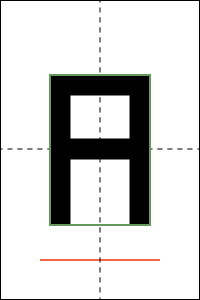
\includegraphics[height=20em]{A.png}
  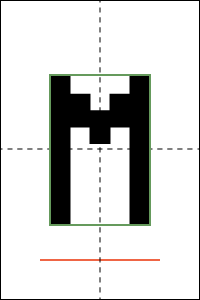
\includegraphics[height=20em]{M.png}
\end{center}


\begin{ayuda}

  \noindent{\bf Notas.}

  \begin{itemize}

    \item Use un reticulado con $h\sim0.2~{\rm [cm]}$.

    \item Use el método de sobre-relajación sucesiva con distintos $w$ y
      estudie cuantas iteraciones hacen falta para converger en cada caso.

    \item Note que tendrá que derivar el algoritmo de iteración para los puntos
      adyacentes al segmento con condición de borde derivativa y para el
      segmento mismo.  Debido a esto, es recomendable separar la iteración en
      distintos segmentos

    \item Debe definir un criterio de convergencia, explicítelo en el informe.

    \item Parta con un setup simple y vaya agregando complejidad, asegurándose
      primero de que los casos simples funcionan. Vaya dejando el rastro de su
      trabajo en \texttt{git}.

    \item Asegúrese de incluír gráficos que demuestren de forma efectiva la
      solución obtenida. Éstos pueden incluir gráficos de superficie en 2D y
      3D, líneas de contorno, cortes transversales, etc. Note que el efecto de
      la letra es muy tenue (la carga es baja) por lo que debe probar
      alternativas para la escala del plot.

  \end{itemize}


\end{ayuda}


\vspace{2em}
\noindent\textbf{Instrucciones Importantes.}
\begin{itemize}

\item \textbf{NO USE JUPYTER NOTEBOOKS}. Estamos revisando en serio el diseño
  del código por lo que es imprescindible que entregue su código en un archivo
  de texto \texttt{.py}.

\item Evaluaremos su uso correcto de python. Si define una función
  relativametne larga o con muchos parámetros, recuerde escribir el
  \emph{docstring} que describa los parámetros que recibe la función, el
  output, y el detalle de qué es lo que hace la función. Recuerde que
  generalmente es mejor usar varias funciones cortas (que hagan una sola cosa
  bien) que una muy larga (que lo haga todo).  Utilice nombres explicativos
  tanto para las funciones como para las variables de su código. El mejor
  nombre es aquel que permite entender qué hace la función sin tener que leer
  su implementación ni su \emph{docstring}.

\item Su código debe aprobar la guía sintáctica de estilo
  (\href{https://www.python.org/dev/peps/pep-0008/}{\texttt{PEP8}}). Lleva
  puntaje.

\item Utilice \texttt{git} durante el desarrollo de la tarea para mantener un
  historial de los cambios realizados. La siguiente
  \href{https://education.github.com/git-cheat-sheet-education.pdf}{cheat
    sheet} le puede ser útil. {\bf Revisaremos el uso apropiado de la
  herramienta y asignaremos una fracción del puntaje a este ítem.} Realice
  cambios pequeños y guarde su progreso (a través de \emph{commits})
  regularmente. No guarde código que no corre o compila (si lo hace por algún
  motivo deje un mensaje claro que lo indique). Escriba mensajes claros que
  permitan hacerse una idea de lo que se agregó y/o cambió de un
  \texttt{commit} al siguiente.

\item Para hacer un informe completo Ud. debe decidir qué es interesante y
  agregar las figuras correspondientes. No olvide anotar los ejes e incluir una
  \emph{caption} o título que describa el contenido de cada figura. Tampoco
  olvide las unidades asociadas a las cantidades mostradas en los diferentes
  plots.

\item La tarea se entrega subiendo su trabajo a github. Clone este repositorio
  (el que está en su propia cuenta privada), trabaje en el código y en el
  informe y cuando haya terminado asegúrese de hacer un último \texttt{commit}
  y luego un \texttt{push} para subir todo su trabajo a github.

\item El informe debe ser entregado en formato \texttt{pdf}, este debe ser
  claro sin información de más ni de menos. \textbf{Esto es muy importante, no
  escriba de más, esto no mejorará su nota sino que al contrario}. La presente
  tarea probablemente no requiere informes de más de 3 o 4 páginas en total
  (dependiendo de cuántas figuras incluya; esto no es una regla estricta, sólo
  una referencia útil).  Asegúrese de utilizar figuras efectivas y tablas para
  resumir sus resultados. Revise su ortografía.

\end{itemize}

%% FIN ENUNCIADO ===============================================================
%% =============================================================================

\end{document}
